\documentclass{article}
\RequirePackage[a4paper]{geometry}
\geometry{top=25mm,bottom=25mm,left=25mm,right=25mm,nohead,nofoot,includeheadfoot}
\pagestyle{empty}
\usepackage{mathptmx,graphicx}
\usepackage{microtype}
\setlength{\emergencystretch}{1.5em}
\usepackage[dvipsnames]{xcolor}
\usepackage{abstract} % Allows customizing the abstract
\usepackage[numbers,sort&compress]{natbib}
\usepackage{hyperref}
\usepackage[labelfont=bf]{caption}
\usepackage{indentfirst}
\usepackage{amssymb}
\usepackage{amsmath}
\usepackage{diagbox}
\usepackage{svg}
\usepackage{algorithm}
\usepackage{algpseudocode}
\usepackage{wrapfig}
\graphicspath{{figures/}}
\bibliographystyle{unsrt}


\renewcommand{\abstractname}{\Large Abstract}
\begin{document}
\twocolumn[{%
\begin{center}
%{\Large\bfseries
%Transmission estimation in multi-mode fibers using deep neural networks \par}
{\Large\bfseries
Breaking the Phase-Ambiguity Limit: Reference-less 3D Vectorial Transmission-Matrix Retrieval in Multimode Fibers \par}
\vspace{3ex}
{\bfseries
Dvir Marsh$^{1}$, Lior Fridman$^{1}$, Shie Mannor$^{1}$, Guy Bartal$^{1}$\par}
{\footnotesize\itshape
1. Andrew and Erna Viterbi Department of Electrical \& Computer Engineering, Technion, Haifa 3200003, Israel\\
}
\vspace{3ex}
\end{center}

\begin{onecolabstract}
\textbf{
\bfseries
Multimode fibers can carry hundreds of independent spatial channels through a single hair-thin core, making them attractive for ultra-thin endoscopy, targeted light delivery, and space-division multiplexing. Realizing this potential requires knowledge of the fiber's transmission matrix. Interferometric methods recover the phase accurately but rely on a known reference beam and sub-wavelength mechanical stability, while reference-less methods relax these demands at the cost of phase ambiguities that restrict wavefront control to a single plane and a single polarization. Here, we demonstrate reference-less retrieval of the transmission matrix that supports complete three-dimensional and vectorial control of the transmitted field. The approach embeds prior knowledge of the fiber's guided modes into the retrieval itself, which eliminates the ambiguities that arise in the common use of the pixel basis. Because the retrieved matrix is expressed in the modal basis, the number of measurements is set by the number of guided modes rather than by the larger number of sampled pixels, and reconstruction is completed in seconds. The same modal constraint holds even from a single measurement plane: the retrieved matrix still achieves high-quality control of the transmitted field in the conjugate plane, where no data was recorded, halving the required measurements and simplifying the optical setup. 
}
\end{onecolabstract}
\vspace{3ex}
}]

\section{Introduction}
The technological appeal of multimode optical fibers (MMFs) rests on the fact of a hair-thin core supporting numerous guided modes, packing many optical channels into a minimal footprint \cite{applications_review, puttnam2021}. This capacity underpins several important application domains; in biomedical imaging, for example, an MMF provides an ultra-thin endoscopic conduit for delivering and collecting light deep within tissue, with a probe diameter well below that of conventional fiber-bundle endoscopes \cite{deep_brain_in_vivo,ntziachristos2010, scanner_free, imaging_example, seeing_through_chaos}; in optical communications, the same modes provide parallel transmission channels for space-division multiplexing, a route to fiber capacity beyond the limits of single-mode systems \cite{multiplexing_example, puttnam2021}. To fully exploit the MMF's advantages in these domains, one must effectively predict and control the field transmitted through it. This requires the exact input-output field mapping, manifest in the transmission matrix (TM) - a complex matrix acting on the coefficients of its basis elements. 

The most common basis for TM retrieval is the pixel basis, which complies with the instruments that shape and record the field. As MMFs scramble both spatial and polarization degrees of freedom (DOF) \cite{xiong2017}, a complete formulation of the TM in the pixel basis requires a vectorial representation \cite{tripathi2012}. Acquiring such a vector TM necessitates access to the phase of the transmitted field, conventionally obtained by interfering it with an external reference arm \cite{seeing_through_chaos, yu2013}, and repeating the measurement for both output polarizations \cite{tripathi2012, xie2017}. However accurate, this measurement rests on a reference field that must be known precisely and held stable to a fraction of a wavelength throughout the acquisition, with a path length matched to the signal within the coherence length of the source \cite{goodman2015}. Such stability is routine on an isolated optical bench, yet out of reach in the very settings that motivate MMFs: an endoscope bending inside tissue, or a multiplexing link deployed outside the laboratory.

These requirements can be relaxed by deriving the reference beam from the light that already propagates through the fiber, or by eliminating the reference altogether. In common-path schemes, part of the input degrees of freedom is used as a reference, such that it shares a common path with the signal so the measurement becomes insensitive to global drift \cite{florentin2018, jakl2022, TM_Gigan, yoon2015}. Reference-less take another step, recovering the TM from intensity-only measurements by phase retrieval and omitting the interferometer entirely \cite{dremeau2015, mode_control, nonconvex_opt}. In either case, the transmitted phase is no longer referred to a known field: the co-propagating reference carries its own unknown speckle phase \cite{jakl2022}, while intensity detection in a single plane discards the phase between output pixels \cite{dremeau2015}. Both therefore recover the matrix only up to a row-dependent phase offset, with one unknown phase per output pixel. These offsets reproduce the correct intensity pattern in the calibration plane, but propagating the field away from it returns the wrong solution, restricting control to a single plane. Recent reference-less variants constrain the offsets with a second measurement plane, restoring propagation at the cost of a larger measurement budget and slower acquisition \cite{zhong2023, retrieving_the_complex_TM}. Others extend the retrieval to both input polarizations \cite{wei2026millisecond}. In all of them, the field is detected in a single output polarization, so the retrieved matrix stays scalar, leaving much of the fiber's vectorial capacity unused.

An alternative approach relies on the guided modes of the fiber as the basis for representing the TM. The dimension of the TM is then set by the number of modes, rather than the potentially larger number of pixels used to sample them, thereby lowering the measurement budget. Even so, most modal retrievals remain interferometric, recovering the transmitted field by digital holography against an external reference\cite{rothe2019, li2021}. The only reference-less realization excites the modes one at a time and reads them out through a correlation filter \cite{bruning2015}, which cannot be scaled for thousands of modes, due to alignment limitations and filter capacity. Moreover, most of these methods assume scalar fields \cite{rothe2019, li2021, bruning2015}, and address a single polarization, thus forfeiting half the fiber's capacity.

Full control over the field outside the laboratory requires a retrieval process possessing the compactness and vectorial reach of the modal basis without relying on sensitive and complicated additions such as interferometer.

Here, we experimentally demonstrate for the first time, to our knowledge, a reference-less full TM retrieval over a MMF supporting $M=1508$ modes. We embed \textit{a priori} constraints of the guided modes directly into the retrieval process, by expressing each output field as a superposition of globally supported vector modes, leading to three significant advantages: First, these constraints lift the row-wise phase ambiguity of conventional single-plane retrieval. Second, the modes' structure allows for vectorial control over the output, without the need for an additional polarizer. And last - due to the reduced number of the required DoFs ,compared to those required in the pixel basis, the retrieval converges faster and requires fewer measurements than state-of-the-art reference-less methods. Altogether, this method brings complete field control with reduced physical and computational requirements, paving the way for real-world MMF applications such as endoscopes and optical transceivers.

\section{Results}
We retrieve the TM directly in the modal basis, formed by the $M=1508$ guided modes of the fiber.
Each mode is a vector eigenmode of the wave equation for the fiber's step-index profile \cite{fiber_book}.
Its transverse amplitude, phase, and polarization profiles can therefore be computed in advance and serve as constraints on the retrieval.

In an ideal straight fiber, the TM is diagonal in the modal basis: each mode propagates independently, acquiring only a mode-dependent phase.
In practice, however, core ellipticity, stress, and bending couple the guided modes, populating the off-diagonal elements of the TM and redistributing power among the modes \cite{xiong2017}.
The TM, which captures this coupling, is inferred from output measurements recorded for a set of known input wavefronts.

In our reference-less scheme, these measurements are intensity images recorded by polarization-insensitive cameras, $I=|E_x|^2+|E_y|^2$.
The intensity at pixel $n$ does not change if the local field vector $\mathbf{E}_n$ is multiplied by a phase factor and its polarization is rotated, $\mathbf{E}_n\to e^{i\phi_n}R(\theta_n)\mathbf{E}_n$.
Applying this transformation to the two rows of a vector pixel-basis TM that belong to pixel $n$ therefore leaves every recorded image unchanged.
A single-plane, pixel-basis retrieval thus recovers the TM only up to an independent phase $\phi_n$ and rotation $\theta_n$ at each pixel.
We refer to these as the local phase ambiguity and the local polarization-orientation ambiguity.
The former is the row-wise phase ambiguity of pixel-basis methods \cite{dremeau2015, nonconvex_opt}, which restricts control to the calibration plane unless a second plane is recorded \cite{zhong2023, retrieving_the_complex_TM}.
The latter leaves the orientation of the retrieved $x$ and $y$ axes undetermined at each pixel.
This prevents vectorial control, i.e., independent control of both output polarization components, unless the polarizations are separated at detection, as in interferometric vector TM measurements \cite{tripathi2012, xie2017}.

Constraining the field at the output facet to a superposition of the $M$ guided modes lifts both local ambiguities:
\begin{equation}
\label{eq:modal_expansion}
\mathbf{E}(x,y)=\sum_{l=1}^{M} w_l\left(\psi_{l,x}(x,y)\,\hat{x}+\psi_{l,y}(x,y)\,\hat{y}\right).
\end{equation}
The $2N$ complex amplitudes of the two field components on $N$ camera pixels are replaced by $M$ modal coefficients $w_l$, each weighting a known vector profile $(\psi_{l,x},\psi_{l,y})$.
These profiles span only an $M$-dimensional subspace of the $2N$-dimensional space of sampled fields.
A transformation that varies from pixel to pixel therefore generally maps a superposition of guided modes to a field outside this subspace, which Eq.~\eqref{eq:modal_expansion} cannot represent.
Only a transformation that is the same at every pixel within the core, $\phi_n=\phi$ and $\theta_n=\theta$, can preserve the subspace.
The $N$ local phases and $N$ local rotations thus reduce to a single global phase and a single global rotation of the polarization axes.
Figures~\ref{fig:cross_plane_focus} and \ref{fig:vector_control} test these two reductions experimentally.

We impose the modal constraint by fitting a forward model of the optical path in Fig.~\ref{fig:setup}, parameterized by the TM, to the measured intensities.
The model computes the field at the fiber input facet from the phase pattern displayed on the spatial light modulator (SLM).
Projecting this field onto the guided modes yields the input modal excitation vector $\mathbf{z}_{\text{in}}\in\mathbb{C}^M$.
The fiber is represented by the TM, $T\in\mathbb{C}^{M\times M}$, which maps $\mathbf{z}_{\text{in}}$ to the output modal vector $\mathbf{w}=T\mathbf{z}_{\text{in}}$.
Using Eq.~\eqref{eq:modal_expansion}, the model then computes the output field in the image plane of the fiber output facet and in its Fourier plane.
It predicts the polarization-summed intensity recorded in each plane by two simultaneously exposed cameras.
We fit $T$ in one of two ways (Methods).
A joint fit estimates $T$ together with the static imperfections of the optics, such as aberrations and misalignment; this calibration of the optics is needed only once per optical alignment.
Afterwards, a fast alternating-direction method of multipliers (ADMM), adapted from Wei \textit{et al.}~\cite{wei2026millisecond} to the modal basis, fits $T$ alone.
Either fit requires only intensity images, recorded with no reference beam and no output polarizer.

\begin{figure*}[t]
\centering
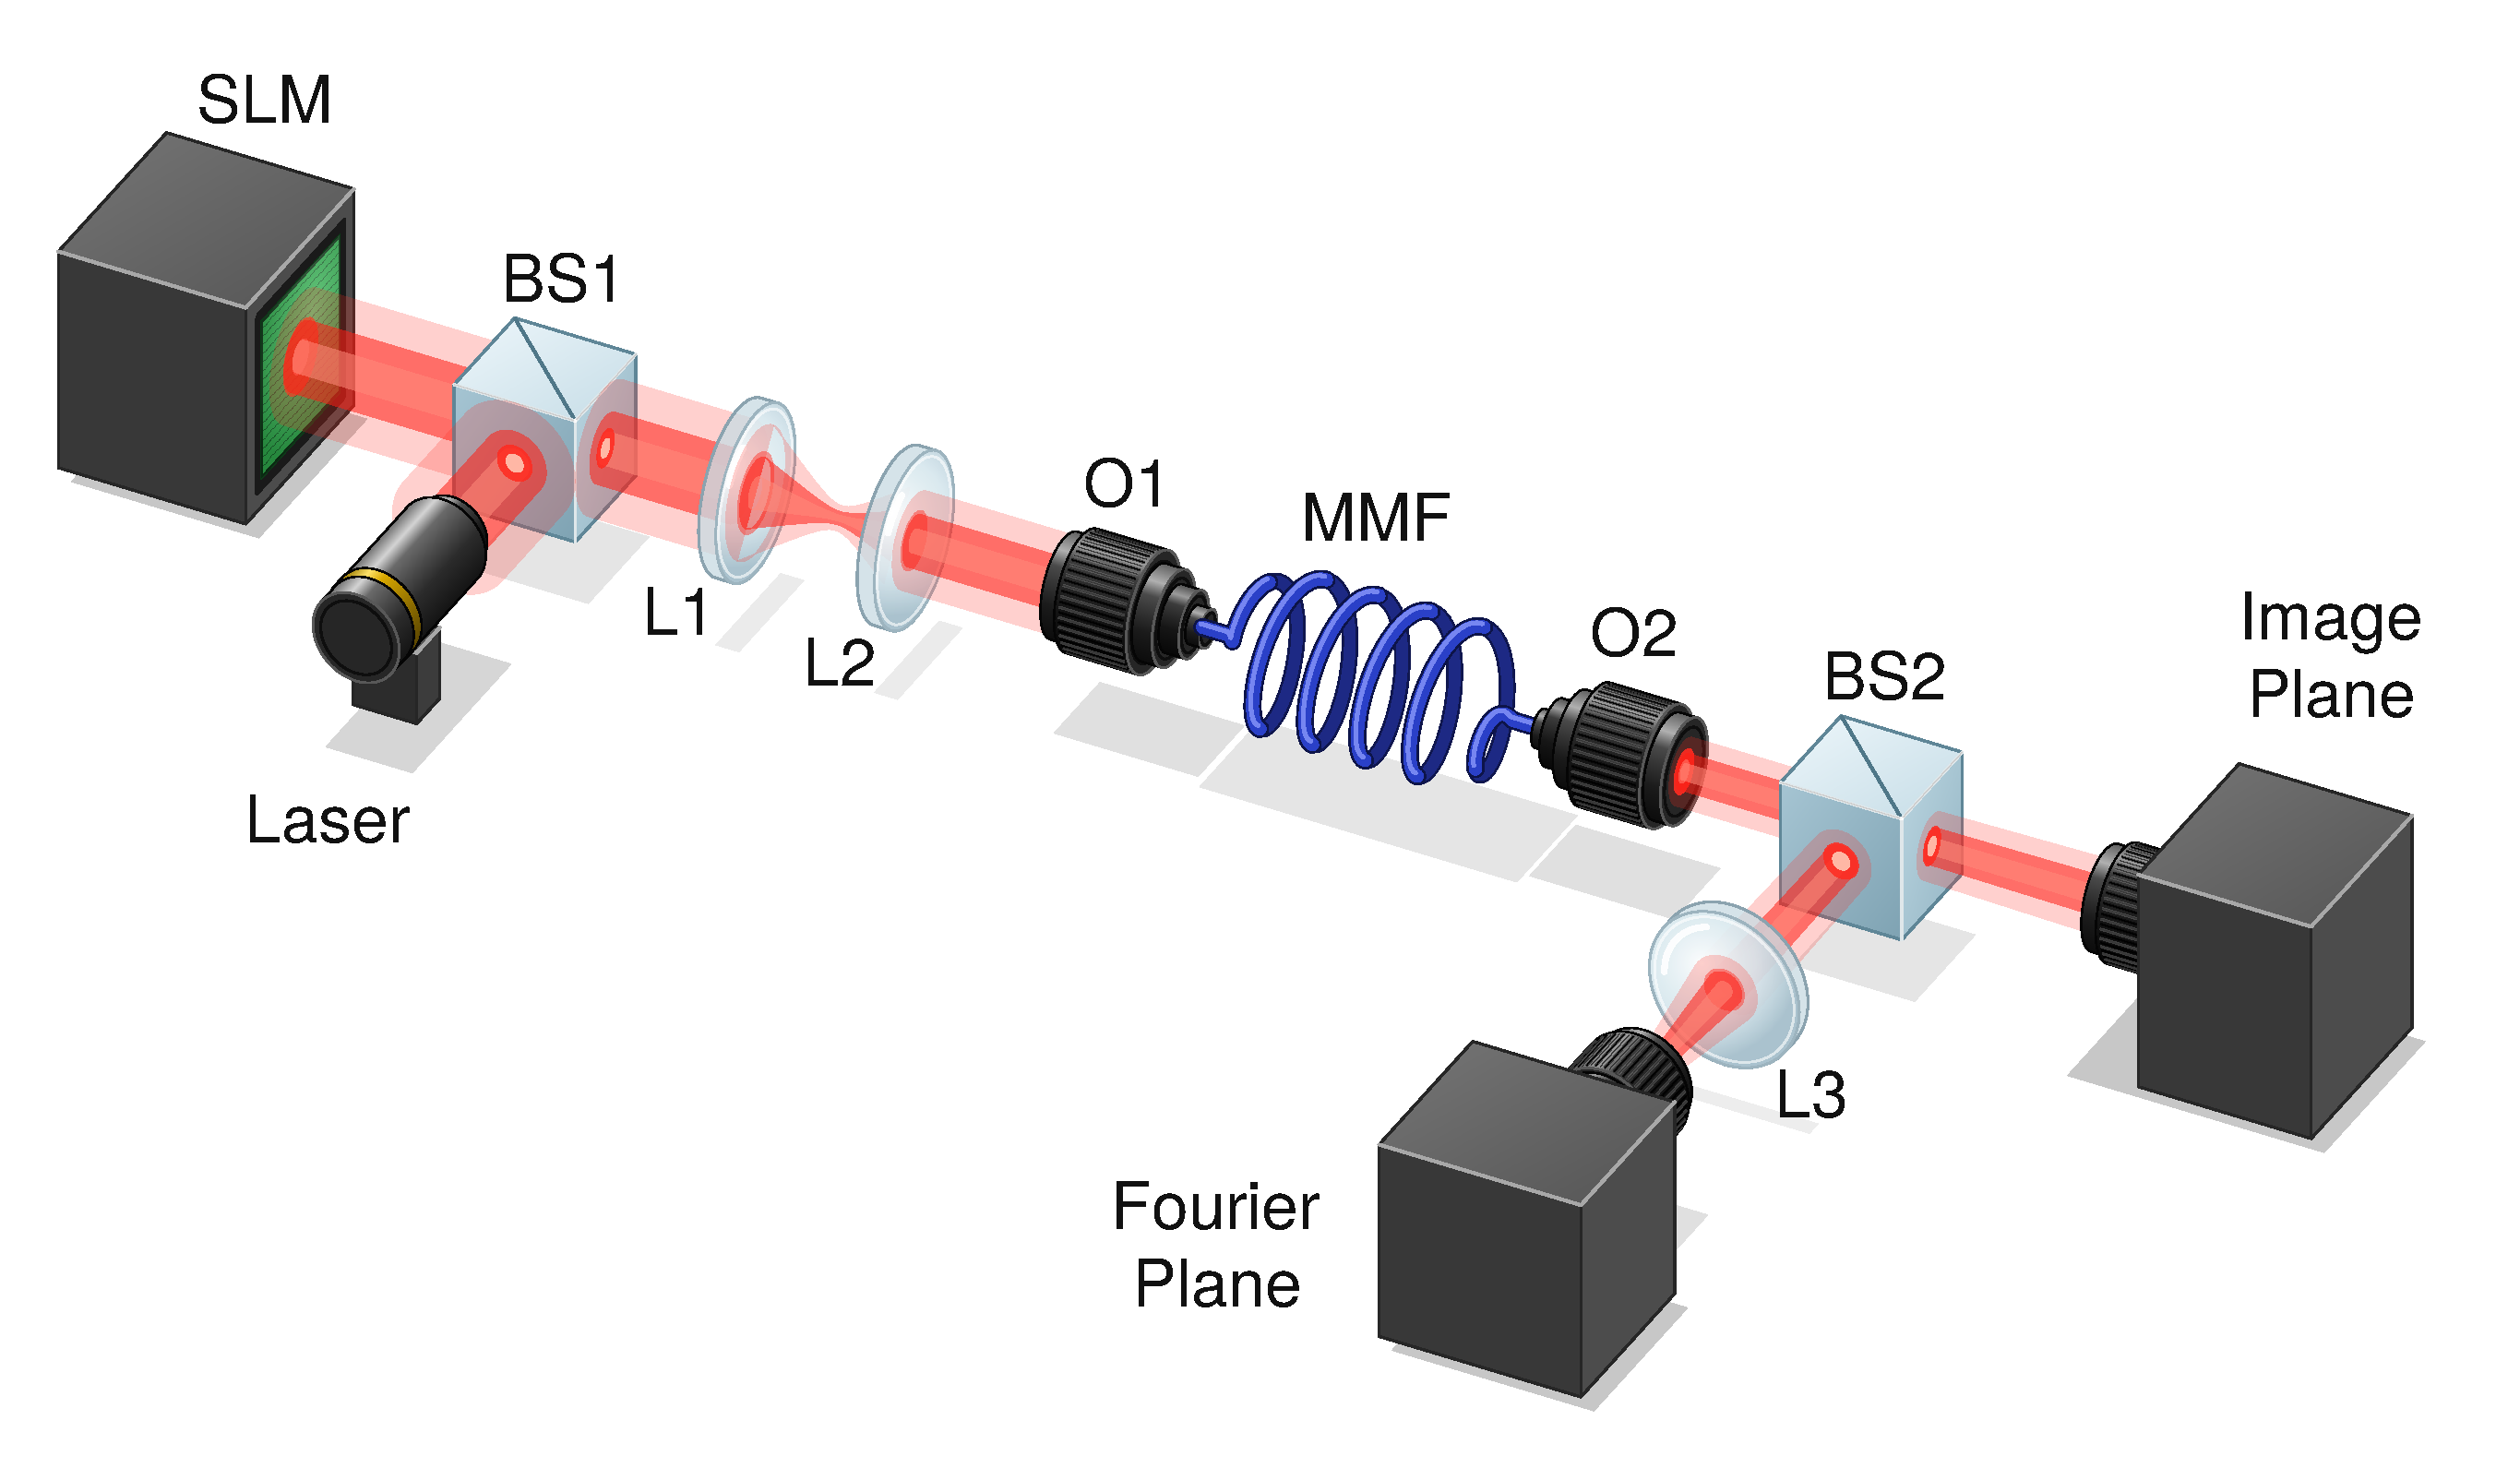
\includegraphics[width=0.85\textwidth]{figures/optical_setup_3d.pdf}
\caption{\textbf{Experimental setup.} A HeNe laser ($\lambda=632.8$\,nm) illuminates a phase-only spatial light modulator (SLM) through beam splitter BS1. The SLM modulates one polarization component of the incident field. Lenses L1 and L2 image the SLM onto the back focal plane of objective O1, which couples the shaped field into the MMF (length 1\,m, core diameter 50\,$\mu$m, $\mathrm{NA}=0.22$, $M=1508$ guided modes). Objective O2 collects the transmitted light, and BS2 splits it between two polarization-insensitive cameras. One camera records the fiber image plane, while the other, placed behind lens L3, records its Fourier plane. Both cameras expose simultaneously for every SLM pattern. No reference arm and no output polarizer are used.}
\label{fig:setup}
\end{figure*}

We start by showing that the modal constraint lifts the local phase ambiguity: a TM retrieved from intensities recorded in one plane enables control of the field in the other (Fig.~\ref{fig:cross_plane_focus}).
For each plane, we retrieved the TM from that plane's intensities alone with the fast ADMM.
We then used it to compute an SLM pattern (Supplementary Material) that focuses light in the other plane.
We quantify focusing by the peak-to-background ratio, $\mathrm{PBR}=I_{\mathrm{peak}}/\langle I\rangle_{\Omega_B}$ \cite{nonconvex_opt}.
Here, $I_{\mathrm{peak}}$ is the intensity of the brightest pixel of the focus, and $\langle I\rangle_{\Omega_B}$ is the mean intensity over the background region $\Omega_B$.
The background region is $\Omega_B=\Omega_F\setminus\Omega_T$, where $\Omega_T$ is the $3\times3$-pixel region centered on the peak ($1.3\times1.3\,\mu\mathrm{m}^2$ in the image plane).
The region $\Omega_F$ is the area the fiber can illuminate: the core in the image plane and the NA-limited disk in the Fourier plane.
With the TM retrieved from Fourier-plane intensities, the measured image-plane focus reached $\mathrm{PBR}=317$ [Fig.~\ref{fig:cross_plane_focus}(a)].
Conversely, with the TM retrieved from image-plane intensities, the Fourier-plane focus reached $\mathrm{PBR}=433$ [Fig.~\ref{fig:cross_plane_focus}(b)].
As discussed above, a single-plane, pixel-basis retrieval would leave the local phases $\phi_n$ undetermined.
The cross-plane focusing therefore shows that the modal constraint determines them up to a global phase.

\begin{figure}[t]
\centering
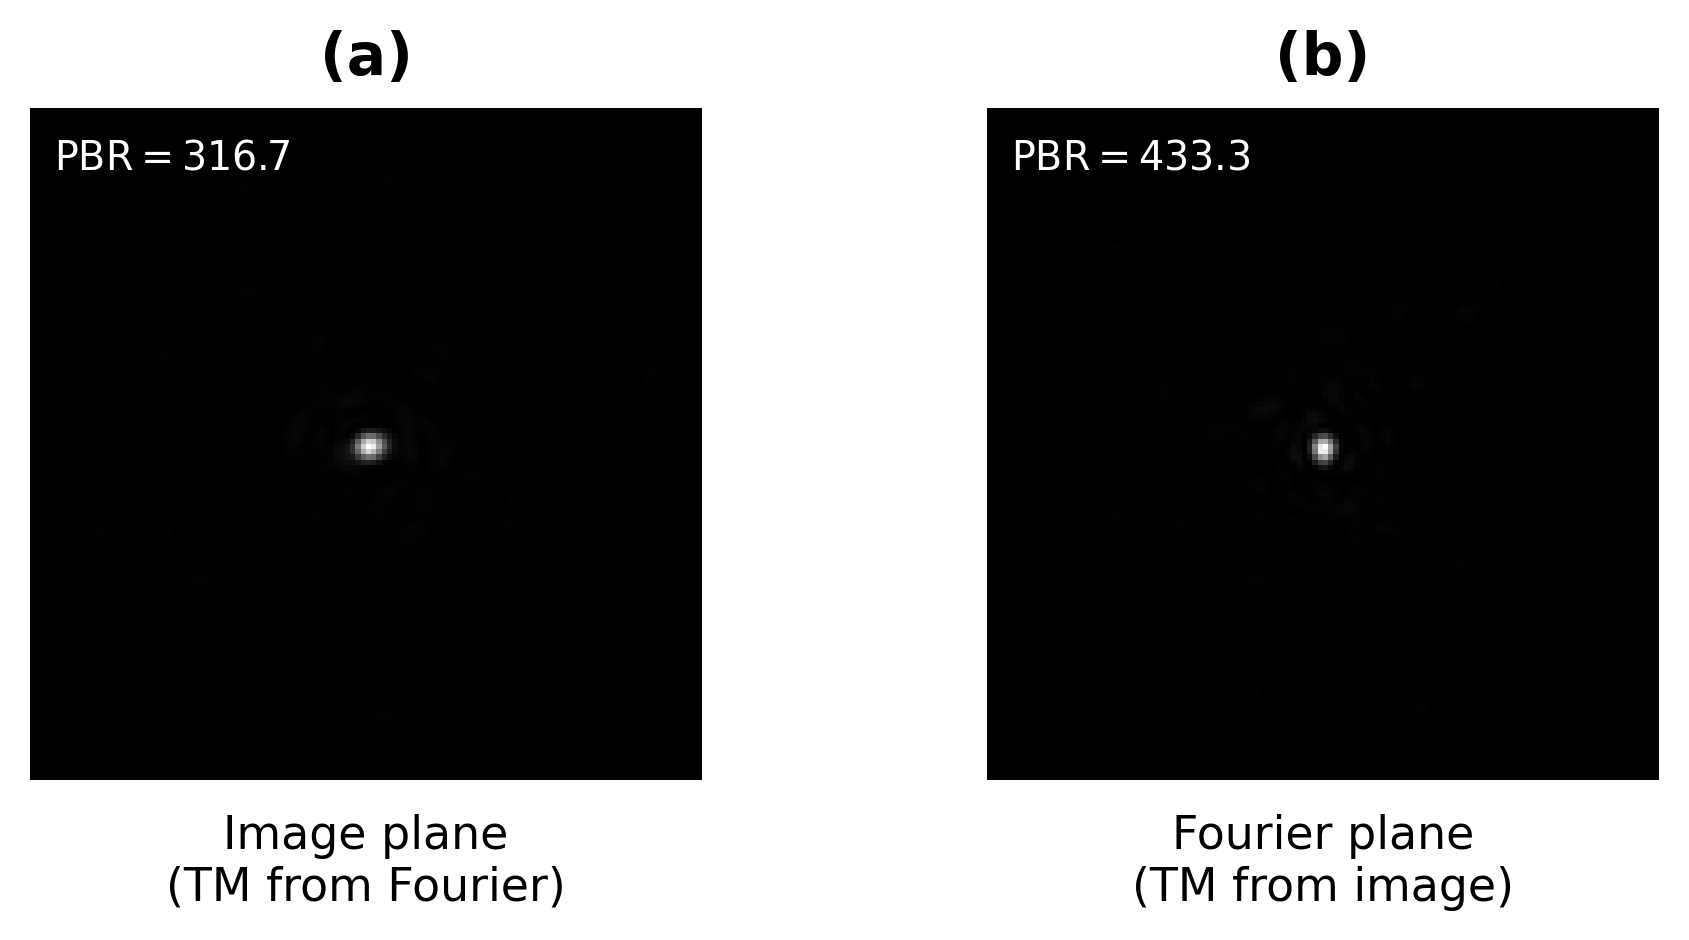
\includegraphics[width=\columnwidth]{figures/tm_cross_plane_focus.png}
\caption{\textbf{Cross-plane focusing following single-plane TM retrieval.} (a)~Image-plane focus obtained with a TM retrieved exclusively from Fourier-plane intensities. (b)~Fourier-plane focus obtained with a TM retrieved exclusively from image-plane intensities. The PBR is indicated in each panel. Both TMs were retrieved by the fast ADMM retrieval (Methods).}
\label{fig:cross_plane_focus}
\end{figure}

The modal constraint also lifts the local polarization-orientation ambiguity, which enables vectorial control without polarization-resolved detection.
We retrieved the TM by the joint fit from polarization-summed intensities, with no polarizer in the detection path.
We then optimized a single SLM pattern to form two spatially separated foci in the image plane, one polarized along each of the retrieved axes, $x'$ and $y'$.
Here, $x'$ and $y'$ denote the two orthogonal polarization axes of the retrieved TM, which are common to all output pixels.
Without a polarizer, the image-plane camera records both foci [Fig.~\ref{fig:vector_control}(a)].
A linear polarizer, placed in front of the camera only for verification, extinguishes either focus while transmitting the other, and the two extinction angles differ by $90^\circ$ [Fig.~\ref{fig:vector_control}(b,c)].
If the retrieved axes varied from pixel to pixel, the difference between the two extinction angles would be arbitrary rather than $90^\circ$.

The single global rotation left by the modal constraint is, however, not fixed by the polarization-summed intensities.
In the weak-guidance approximation, which holds for our fiber ($\mathrm{NA}=0.22$), a uniform rotation of the polarization maps the space spanned by the guided modes onto itself \cite{fiber_book}.
Such a rotation does not change the polarization-summed intensity in either plane.
The retrieved axes $x'$ and $y'$ are therefore rotated from the laboratory axes by an unknown global angle $\theta$.
Because $\theta$ is the same at every pixel, it does not limit vectorial control: the two foci in Fig.~\ref{fig:vector_control} are orthogonally polarized whatever the value of $\theta$.
If the orientation of $x'$ and $y'$ in the laboratory frame is required, the extinction angles of a single linear polarizer give $\theta$ directly [Fig.~\ref{fig:vector_control}(b,c)].

\begin{figure}[t]
\centering
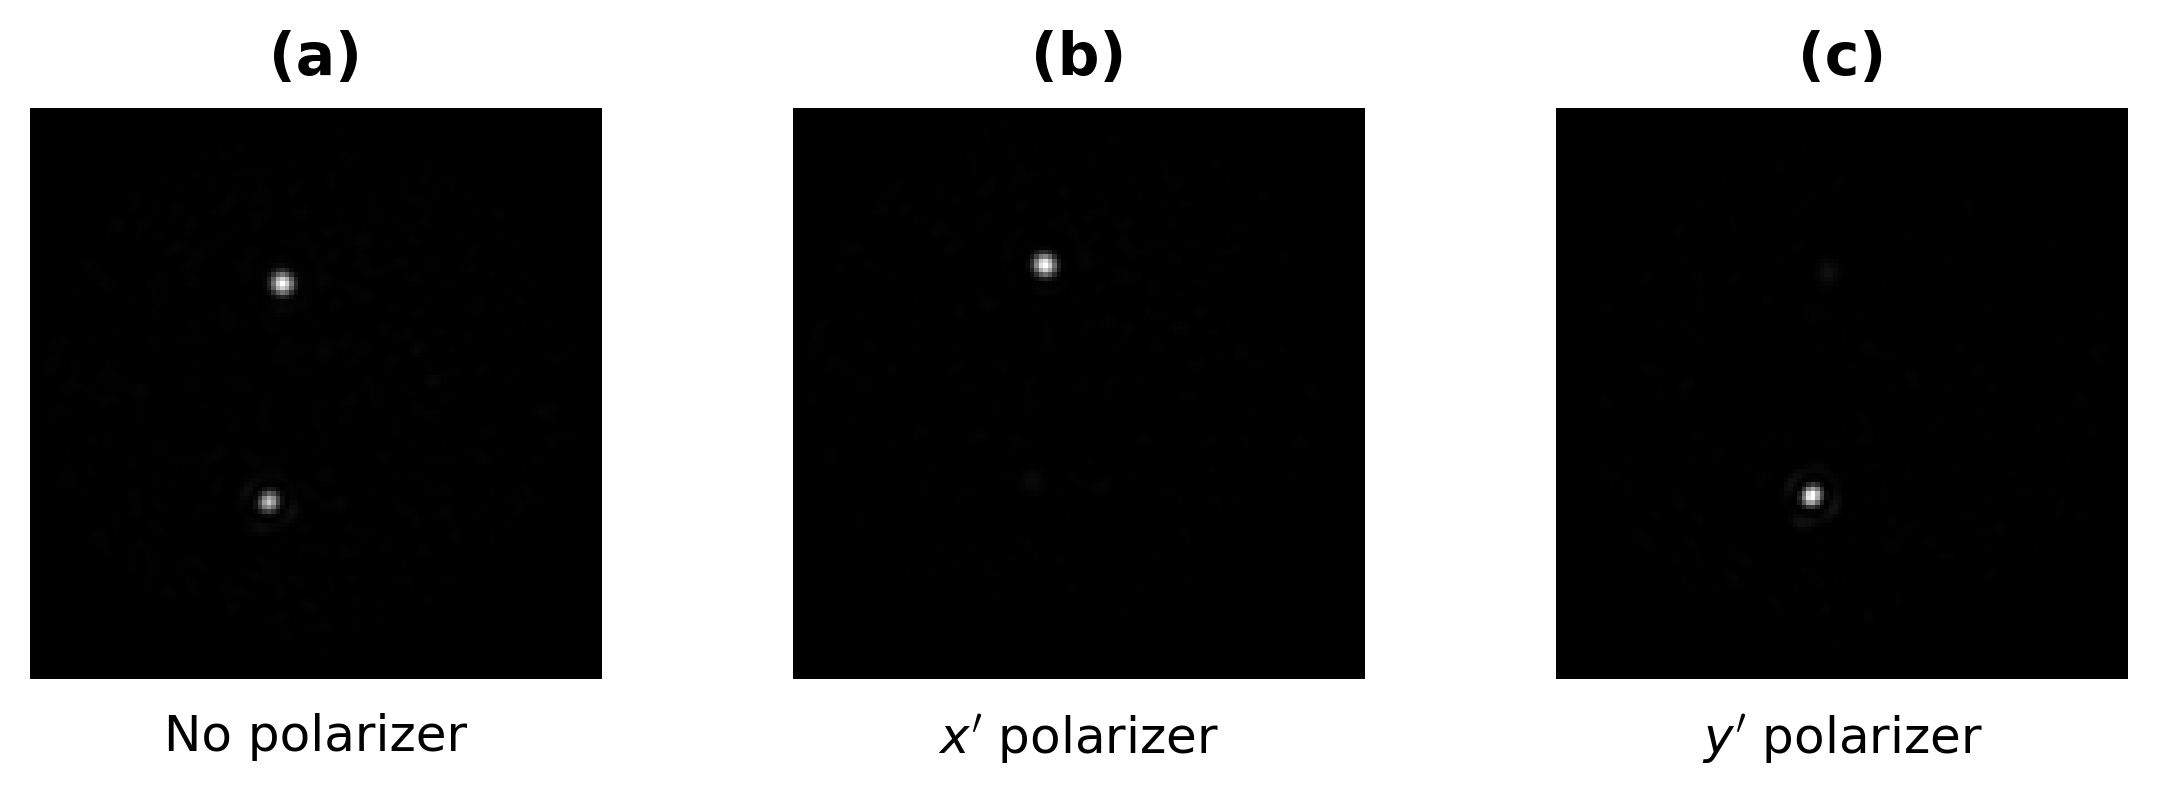
\includegraphics[width=\columnwidth]{figures/tm_vectorial_control.png}
\caption{\textbf{Vectorial focusing and polarization-basis ambiguity.} A single SLM pattern was optimized to produce two spatially separated foci in orthogonal polarization components of the image plane. (a)~With no polarizer, the camera records their summed intensity. (b,c)~A linear polarizer rotated to extinction isolates each focus in turn; the two angles are orthogonal. The TM was retrieved by the joint fit (Methods).}
\label{fig:vector_control}
\end{figure}

Beyond these two tests, we used the retrieved TM to optimize phase-only SLM patterns toward localized, extended, and modal targets in both planes.
A separate SLM pattern was optimized for each plane, except for the modal target.
For these demonstrations (Figs.~\ref{fig:tm_control} and \ref{fig:modal_control}), the TM was retrieved from intensities recorded in both planes.
Although data from a single plane suffice for control (Fig.~\ref{fig:cross_plane_focus}), the second plane adds constraints to the fit and can improve focusing, at no cost in acquisition time.

We first evaluate single-spot focusing [Fig.~\ref{fig:tm_control}(a)].
Across five off-center target positions, the measured PBR is $526\pm71$ in the image plane and $619\pm101$ in the Fourier plane (mean $\pm$ standard deviation).
The foci are also close to the diffraction limit of the fiber: the image-plane focus in Fig.~\ref{fig:tm_control}(a) has a full width at half maximum of $1.57\,\mu$m, compared to $0.514\lambda/\mathrm{NA}=1.48\,\mu$m diffraction limit at $\mathrm{NA}=0.22$.

SLM patterns optimized with the same TM also produce multiple foci simultaneously, at chosen positions within each plane, as shown for three foci in Fig.~\ref{fig:tm_control}(b).
The ratio $\mathrm{PBR}_3$, the mean of the three peak intensities divided by the mean intensity in $\Omega_F$ outside the three $3\times3$-pixel peak regions, is $158$ in the image plane and $181$ in the Fourier plane.
These values are close to one third of the single-spot PBRs ($175$ and $206$), as expected when the intensity concentrated by the optimization is shared among three targets.

We then optimize the SLM phase to form two spatially extended target patterns [Fig.~\ref{fig:tm_control}(c)].
We quantify their fidelity by the Pearson correlation coefficient (PCC) between the measured and target intensities.
For the first pattern, the PCC is $0.926$ in the image plane and $0.857$ in the Fourier plane; for the second, it is $0.922$ and $0.879$, respectively.

\begin{figure*}[t]
\centering
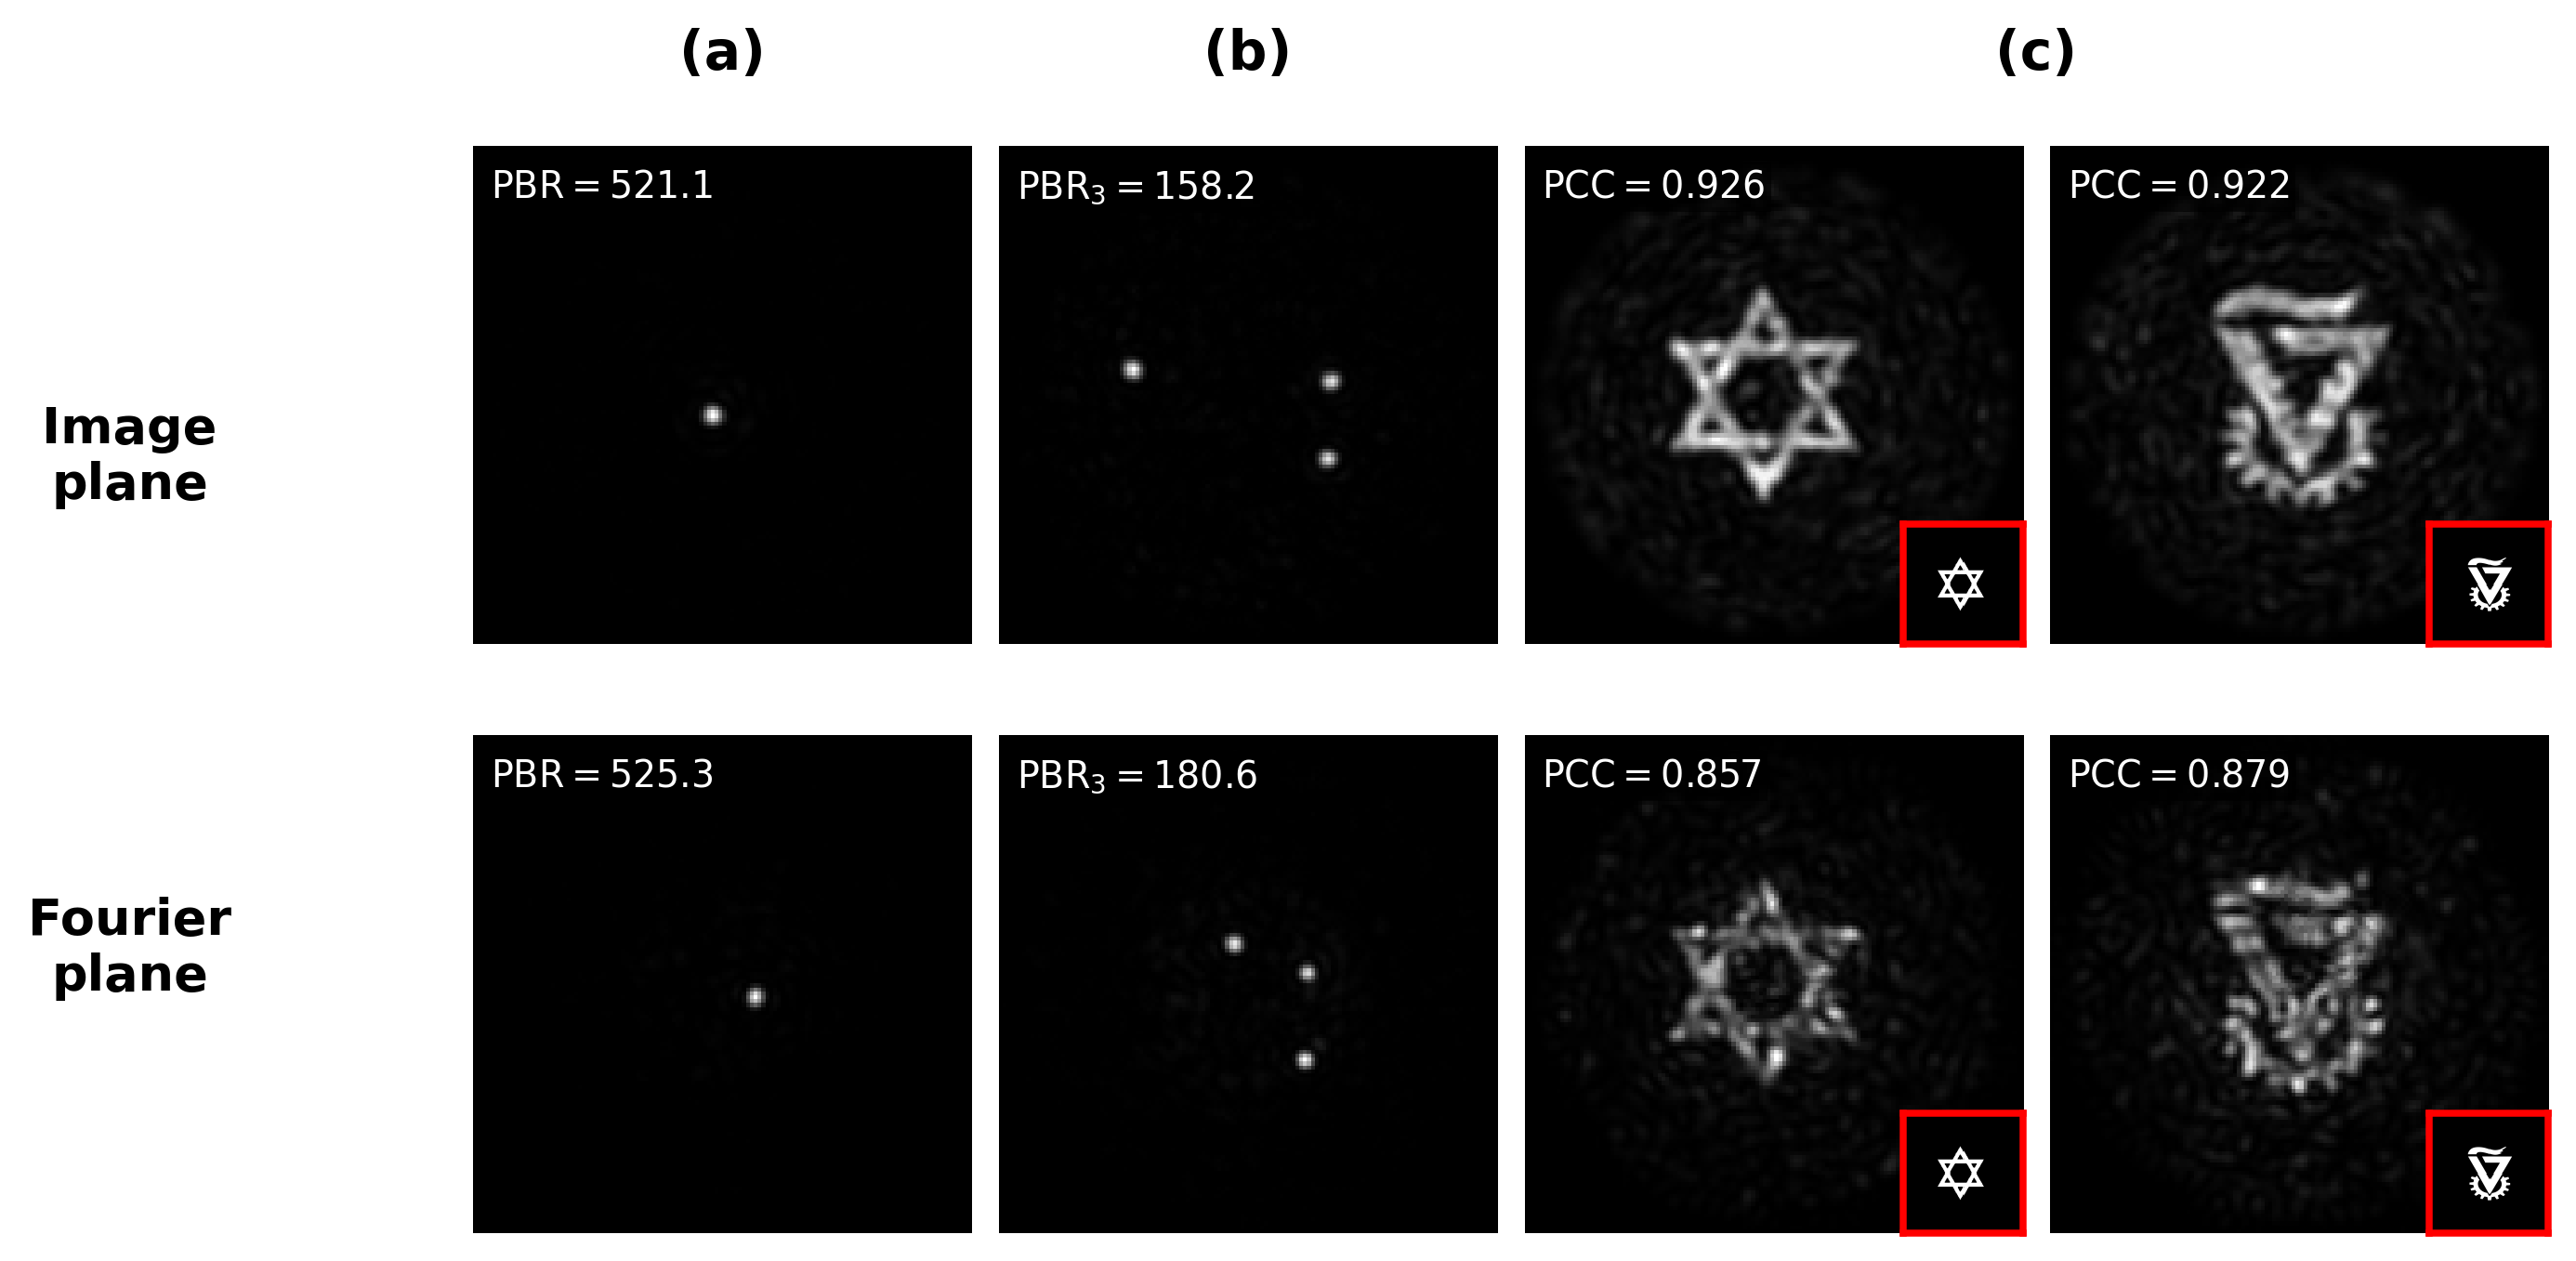
\includegraphics[width=0.85\textwidth]{figures/tm_wavefront_control.png}
\caption{\textbf{Propagation-consistent control of the transmitted field using the retrieved TM.} The first and second rows show intensities recorded in the fiber image and Fourier planes, respectively. (a) Single-spot focusing. (b) Three-spot focusing. (c) Generation of two extended intensity patterns; the prescribed targets are shown as red-bordered insets. Separate plane-specific SLM patterns were used for the image- and Fourier-plane measurements. The TM was retrieved by the joint fit (Methods).}
\label{fig:tm_control}
\end{figure*}

Finally, we optimize an SLM pattern to concentrate the transmitted power into a single guided mode (Fig.~\ref{fig:modal_control}).
A modal target specifies the output modal vector $\mathbf{w}$ itself rather than a field in a particular plane, so one SLM pattern serves both the image- and Fourier-plane measurements.
We quantify the modal purity as the fraction of the transmitted power carried by the target mode $k$, $|w_k|^2/\sum_j|w_j|^2$.
For the $\mathrm{HE}_{8,11}$ mode, the retrieved TM predicts that the optimization raises this fraction from $0.29\%$ for random SLM patterns (mean over 100 patterns) to $79.7\%$.
Because this fraction is predicted rather than measured by an independent modal decomposition, we also compare each recorded intensity pattern with the computed intensity profile of the target mode.
The PCC is $0.891$ in the image plane and $0.895$ in the Fourier plane.
Together, Figs.~\ref{fig:tm_control} and \ref{fig:modal_control} show that the retrieved TM supports single-spot focusing, multi-spot generation, extended-pattern formation, and modal excitation.

\begin{figure}[t]
\centering
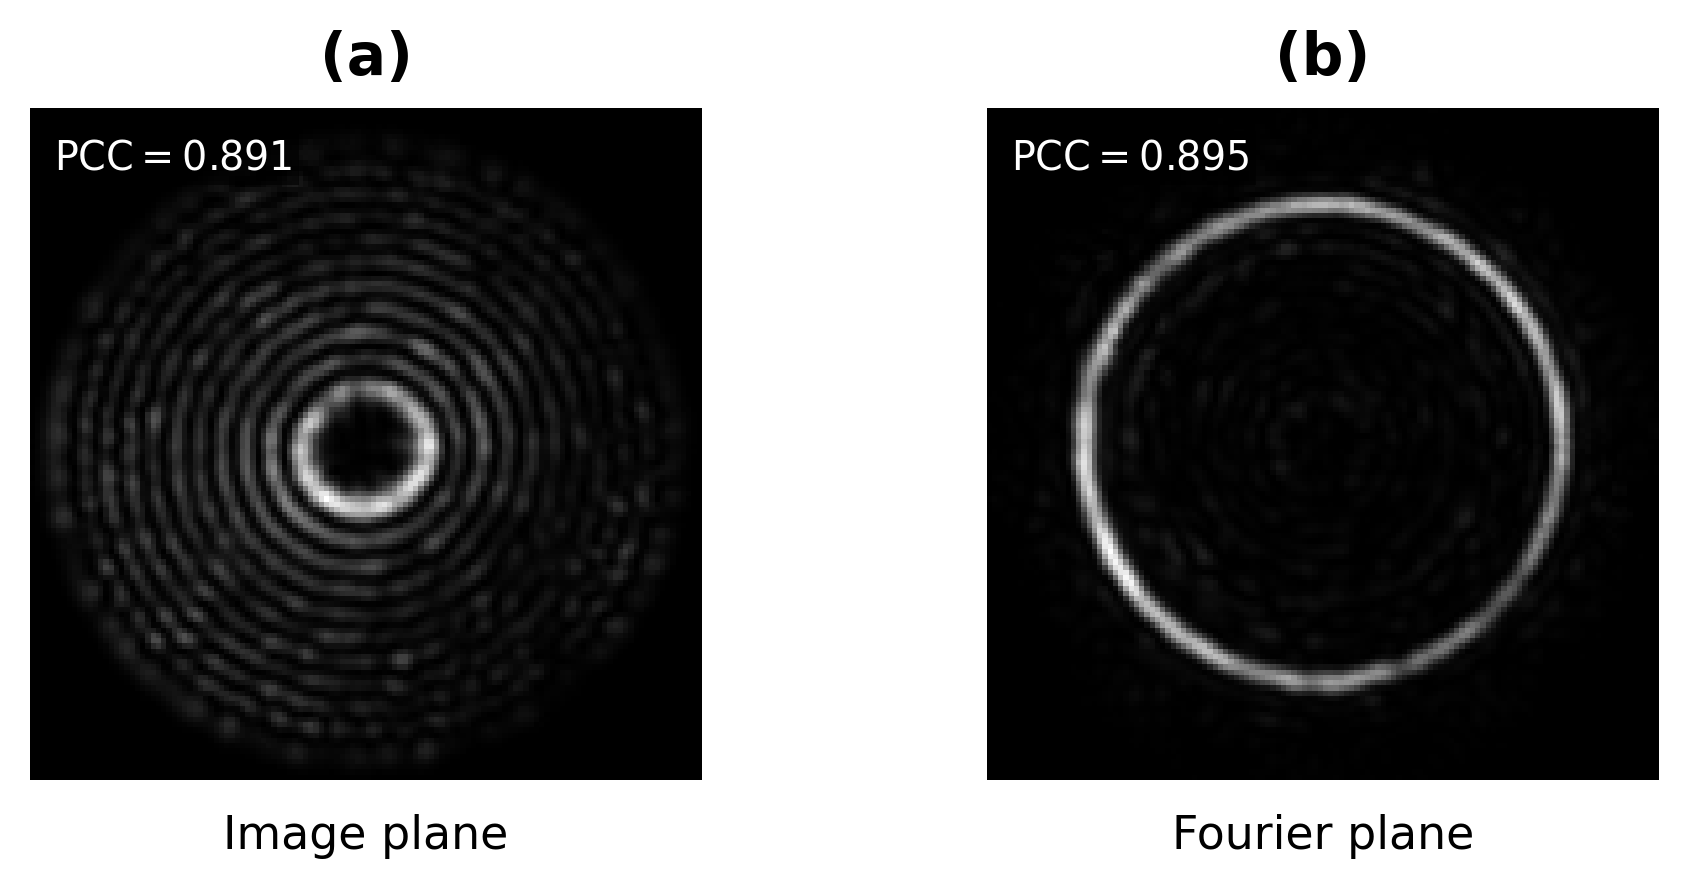
\includegraphics[width=\columnwidth]{figures/tm_modal_control.png}
\caption{\textbf{Selective excitation of a single guided mode using the retrieved TM.} Intensities recorded in (a) the fiber image plane and (b) the Fourier plane for the $\mathrm{HE}_{8,11}$ mode, using the same SLM pattern. The PCC with the intensity profile of the target mode is indicated in each panel. The TM was retrieved by the joint fit (Methods).}
\label{fig:modal_control}
\end{figure}

Representing the TM in the $M$ guided modes rather than on the $N$ camera pixels should reduce both the number of measurements and the computation time required for retrieval.
We test this by measuring the image-plane PBR as a function of reconstruction time (Fig.~\ref{fig:focus_time}).
We compare our modal TM retrieval, using the fast ADMM, with two state-of-the-art reference-less pixel-basis methods: RAF21 \cite{nonconvex_opt} and the pixel-basis ADMM retrieval of Wei \textit{et al.}~\cite{wei2026millisecond}.
All three methods were run with a single modulated input polarization.
Both baselines, as implemented here, retrieve the TM for a single output polarization, so their data were recorded in a separate acquisition, with a linear polarizer in front of the image-plane camera.

The benchmark spans four measurement budgets, $1.2M$, $1.5M$, $2M$, and $3M$ SLM patterns (1809 to 4524 patterns).
Each budget counts displayed SLM patterns, which the two cameras record simultaneously; the dual-plane data of the modal retrieval therefore take no longer to acquire than the baselines' single-plane data.
Performance was quantified by the PBR at a fixed central target position, averaged over ten trials that each draw a different random subset of the recorded patterns.
We report the reconstruction time at which the mean PBR first reaches 500.
The reported times cover the TM optimization alone, excluding the acquisition and the one-time calibration of the optics (Methods).
All retrieval methods ran on the same workstation (12th-generation Intel Core i9 CPU, NVIDIA RTX 3090 GPU).

The modal TM retrieval exceeded $\mathrm{PBR}=500$ at every measurement budget, after 4.73--6.56~s, depending on the budget.
RAF21 crossed this threshold only at $3M$, after 16.26~s; among the tested budgets, the modal retrieval thus reached it with 2.5 times fewer SLM patterns ($1.2M$ versus $3M$).
Pixel-basis ADMM remained below the threshold throughout the measured time window.
Beyond speed and measurement count, only the modally retrieved TM, among the three, enables control of both orthogonal polarizations and both planes from polarization-summed data (Figs.~\ref{fig:cross_plane_focus} and \ref{fig:vector_control}).
The baselines, as implemented here, return a scalar pixel-basis TM that describes a single output polarization, and only in its calibration plane.

\begin{figure}[t]
\centering
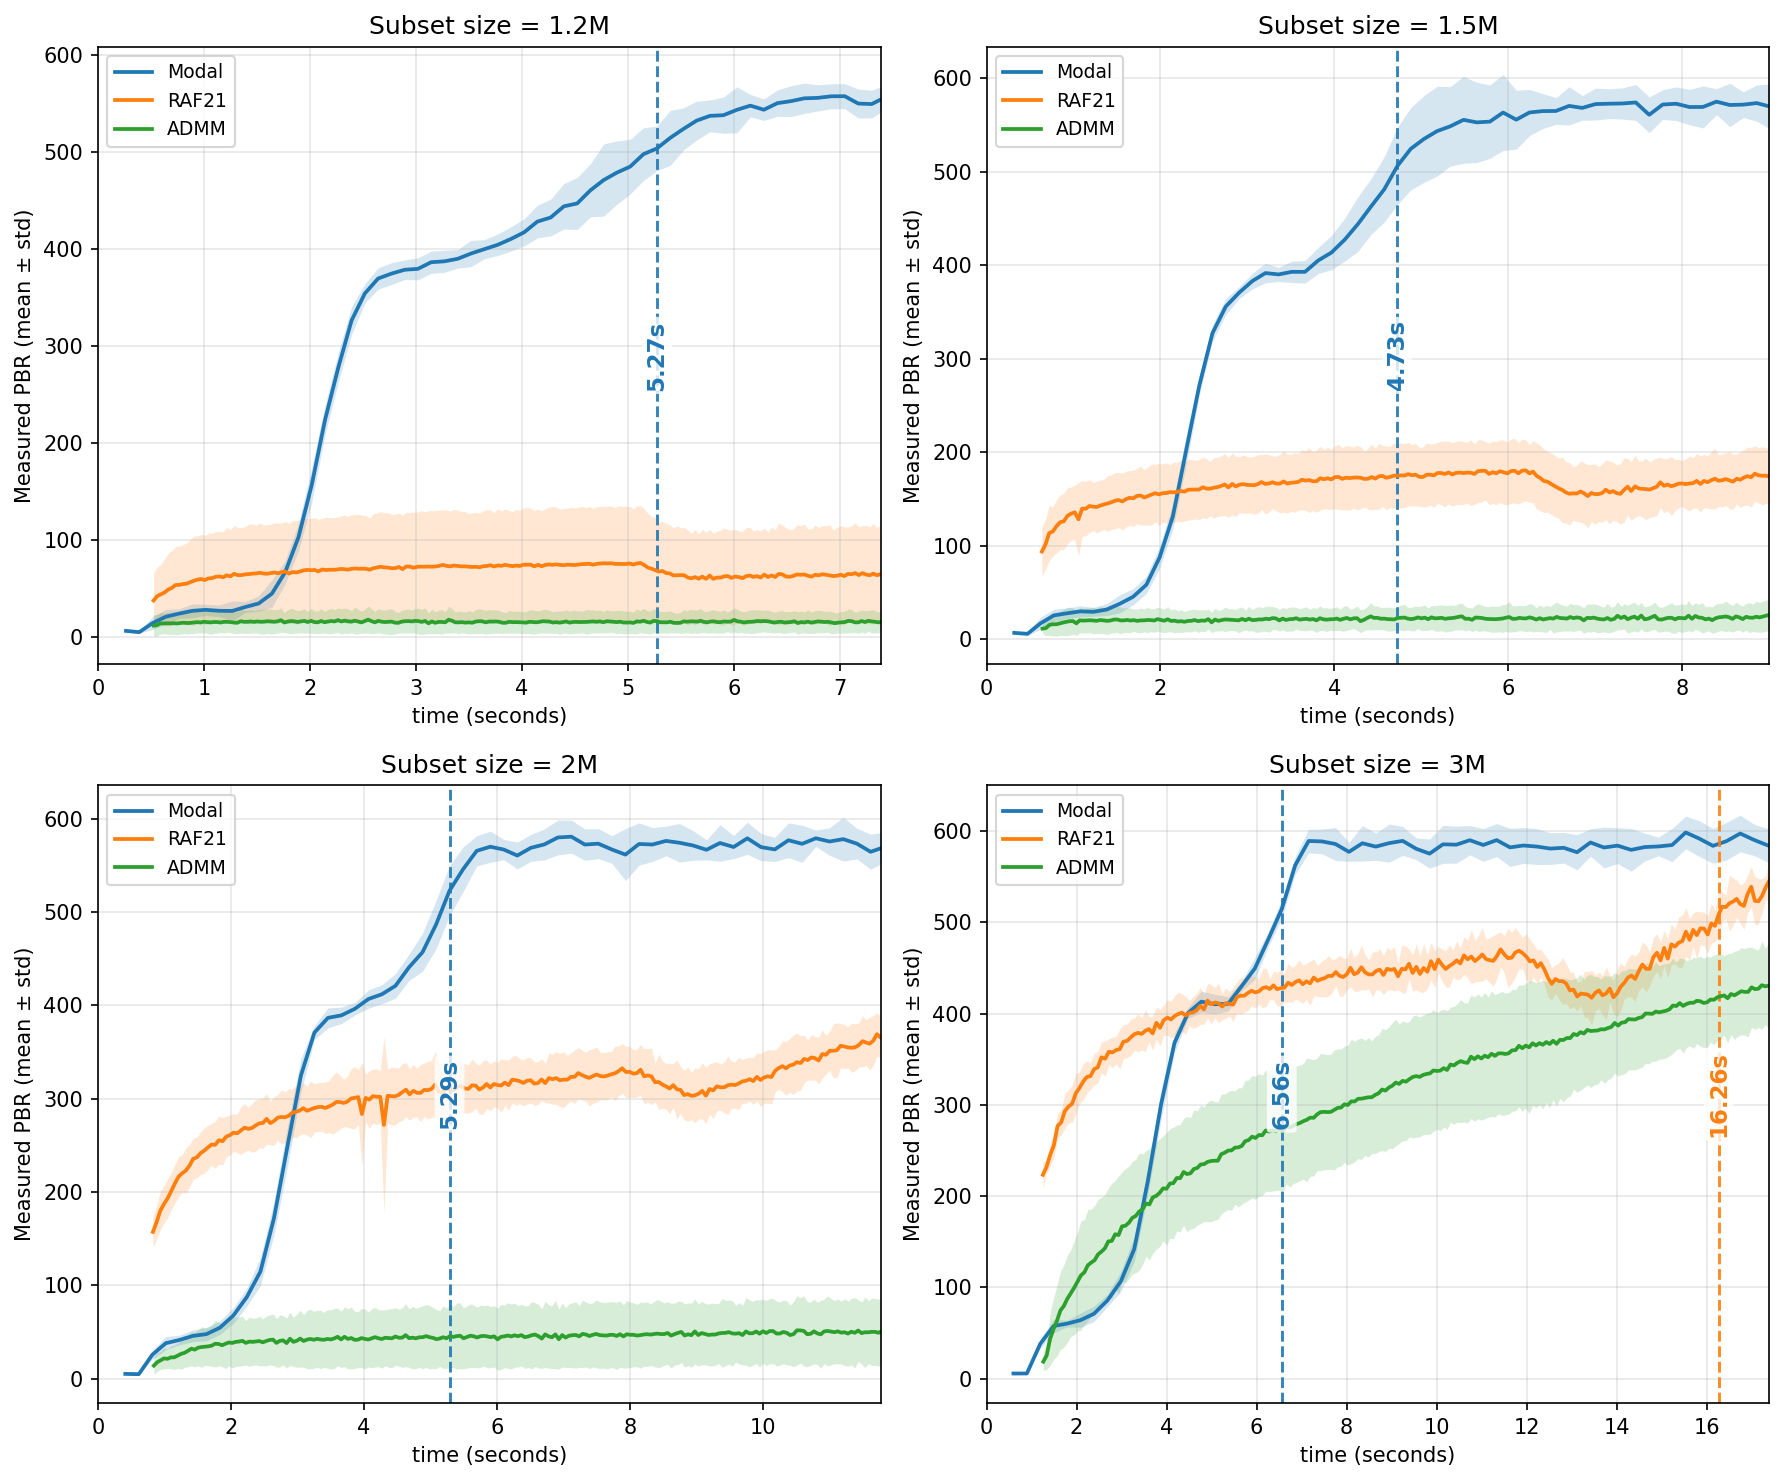
\includegraphics[width=\columnwidth]{figures/lab_focus_vs_accumulated_time.png}
\caption{\textbf{Measured image-plane focusing performance versus reconstruction time.} Results are shown for modal TM retrieval (fast ADMM retrieval, Methods), RAF21 \cite{nonconvex_opt}, and pixel-basis ADMM \cite{wei2026millisecond} at four measurement budgets, expressed relative to the number of guided modes $M=1508$. Curves and shaded regions denote the mean and standard deviation of the PBR over ten trials. Vertical dashed lines mark the first time at which the mean PBR reaches 500. Timing excludes optical acquisition.}
\label{fig:focus_time}
\end{figure}

\section{Methods}
\subsection{Forward Model}
Our forward model follows the optical path of Fig.~\ref{fig:setup} to predict the image- and Fourier-plane intensities produced by a given SLM pattern.
A phase pattern $\Phi(x,y)$ on the SLM modulates one polarization component of the incident field $\mathbf{E}_{\text{inc}}=E_{\text{inc},x}\hat{x}+E_{\text{inc},y}\hat{y}$, resulting in $\mathbf{E}_{\text{SLM}} = E_{\text{inc},x}\exp(i\Phi)\hat{x} + E_{\text{inc},y}\hat{y}$.
The SLM is imaged onto the back focal plane of the input objective, so propagation to the fiber facet is modeled as a Fourier transform of $\mathbf{E}_{\text{SLM}}$.
Projecting the facet field onto the guided modes yields the input modal excitation vector $\mathbf{z}_{\text{in}} \in \mathbb{C}^M$.
The transmission through the fiber is modeled as a linear mixing by the complex-valued TM, $\mathbf{w} = T \mathbf{z}_{\text{in}}$.

We denote by $P_{c,p}$ the linear projection from the modal basis to the pixels of plane $p$ for component $c \in \{x, y\}$, so the predicted field is $E_{c,p}(x,y) = P_{c,p} \mathbf{w}$.
The cameras are polarization-insensitive and the two components are orthogonal, so the observable is the sum of their intensities:
\begin{equation}
I_{\text{pred}, p}(x, y) = |E_{x,p}(x, y)|^2 + |E_{y,p}(x, y)|^2.
\end{equation}

\subsection{Fast TM Retrieval Algorithm}
Recovering the TM from intensity-only measurements is a phase retrieval problem, and polarization-summed detection compounds it: each camera pixel constrains only $I_{\text{meas},p} = |E_{x,p}|^2 + |E_{y,p}|^2$, so no measurement isolates either field component.
We acquire $K$ measurements, one per projected SLM pattern, with the two cameras exposing simultaneously so that every pattern yields an image- and a Fourier-plane frame.
The corresponding modal excitation vectors form the columns of the input probing matrix $Z_{\text{in}} = [\mathbf{z}_{\text{in}}^{(1)}, \dots, \mathbf{z}_{\text{in}}^{(K)}] \in \mathbb{C}^{M \times K}$, where $M$ is the number of guided modes.

We solve for $T$ with an alternating direction method of multipliers (ADMM), adapting the pixel-basis scheme of Wei \textit{et al.} \cite{wei2026millisecond} to the modal basis, to two simultaneously fitted measurement planes, and to polarization-summed data.
ADMM splits the non-convex problem in two: rather than minimizing the intensity residual in $T$ directly, we introduce auxiliary fields $U_{c,p}$, one complex field per polarization component $c$, plane $p$, and probe, and alternate between enforcing the linear physics of propagation, which updates $T$, and enforcing the measured intensities, which updates $U_{c,p}$.
Both subproblems have closed-form solutions, so no gradient-based inner loop is required.
Dual variables $\Lambda_{c,p}$ couple them, accumulating the mismatch between the physically predicted and the measurement-constrained fields so that any inconsistency the physics update cannot absorb is fed back with growing weight.
We start from the straight-fiber prior $T_0 = \mathrm{diag}(e^{i\beta_l L}) + \Delta$, the TM of an ideal, uncoupled fiber, with $\beta_l$ the propagation constant of mode $l$, $L$ the fiber length, and $\Delta$ a complex Gaussian perturbation of standard deviation $0.01$; the dual variables start at zero.

The algorithm proceeds through three sequential steps per iteration (Algorithm~\ref{alg:tm_retrieval}):

\textbf{Step 1: Analytic TM Update (Physics Constraint).}
The TM is updated to the matrix minimizing the model consistency error against the current field estimates:
\begin{equation}
\label{eq:tm_update}
T = \arg\min_{\tilde{T}} \sum_{c,p} \kappa_p \| P_{c,p} \tilde{T} Z_{\text{in}} - (U_{c,p} - \Lambda_{c,p}) \|_F^2.
\end{equation}
The plane weights $\kappa_p = 1/\langle I_{\text{meas},p} \rangle$, the reciprocal mean measured intensity of plane $p$, keep the image and Fourier planes contributing comparably despite their different recorded intensities.
Being a linear least-squares problem, Eq.~\eqref{eq:tm_update} has a closed-form solution (Supplementary Materials), so the TM update is exact and requires no inner iteration of its own.

\textbf{Step 2: Amplitude Projection (Measurement Constraint).}
Next, we obtain the predicted electric fields $E_{c,p} = P_{c,p} T Z_{\text{in}}$ and drive their amplitudes toward the measurement $\sqrt{I_{\text{meas},p}}$.
Because the cameras record the polarization sum, this projection cannot act on $E_{x,p}$ and $E_{y,p}$ separately; it acts jointly, through the combined magnitude of the predicted fields and dual variables,
\begin{multline}
D_{\text{mag},p}(x,y) = \\ \sqrt{|E_{x,p}(x,y) + \Lambda_{x,p}(x,y)|^2 + |E_{y,p}(x,y) + \Lambda_{y,p}(x,y)|^2},
\end{multline}
rescaling both components element-wise by the same real factor:
\begin{multline}
\label{eq:projection}
U_{c,p}(x,y) = \left( \frac{\sqrt{I_{\text{meas},p}(x,y)} + \rho D_{\text{mag},p}(x,y)}{(1+\rho)D_{\text{mag},p}(x,y)} \right) \\ \big( E_{c,p}(x,y) + \Lambda_{c,p}(x,y) \big).
\end{multline}
The measured amplitude is thereby divided between the two components in proportion to their current amplitudes, leaving their relative phase untouched: how the power splits between $E_{x,p}$ and $E_{y,p}$ is set by the vector mode profiles in $P_{c,p}$, not by the data.
This is what allows the vectorial TM to be retrieved with no polarizer in the detection path (Fig.~\ref{fig:vector_control}).
The relaxation parameter $\rho$ sets how far each iteration moves toward the measured amplitude: $\rho = 0$ replaces the predicted magnitude outright, while $\rho > 0$ takes a partial step.
We use $\rho = 0$ for the first $45$ iterations and $\rho = 0.1$ thereafter, chosen empirically: the hard projection descends fastest at first, while the partial step reaches a lower final residual.

\textbf{Step 3: Error Feedback (Dual Update).}
Finally, the dual variables accumulate the residual mismatch between the physically predicted fields $E_{c,p}$ and the measurement-constrained fields $U_{c,p}$,
\begin{equation}
\label{eq:dual_update}
\Lambda_{c,p} \gets \gamma_t \big( \Lambda_{c,p} + E_{c,p} - U_{c,p} \big),
\end{equation}
with $\gamma_t = 0.8^{\lfloor t/15 \rfloor}$ at iteration $t$.
At $\gamma_t = 1$ this is the standard ADMM dual update, an exact integrator of the residual; the periodic decay makes it leaky, stabilizing the optimization landscape and decreasing fluctuations.

\begin{algorithm*}[t]
\caption{Fast ADMM TM Retrieval in the Modal Basis}
\label{alg:tm_retrieval}
\begin{algorithmic}[1]
\State \textbf{Input:} Measured intensities $I_{\text{meas},p}$, input probing matrix $Z_{\text{in}}$, mode projections $P_{c,p}$
\State \textbf{Precompute:} plane weights $\kappa_p = 1/\langle I_{\text{meas},p}\rangle$ and the iteration-independent operators of the Step-1 solution
\State \textbf{Initialize:} $T_0 = \mathrm{diag}(e^{i\beta_l L}) + \Delta$ (straight-fiber prior); auxiliary fields $U_{c,p}$ by one forward pass and projection; dual variables $\Lambda_{c,p} \gets 0$
\For{iteration $t = 1, 2, \dots$}
    \State \textbf{Step 1: TM Update (Physics)}
    \State \quad $T \gets \arg\min_{\tilde{T}} \sum_{c,p} \kappa_p \| P_{c,p} \tilde{T} Z_{\text{in}} - (U_{c,p} - \Lambda_{c,p}) \|_F^2$ \Comment{closed form; Supplementary Materials}
    \State \textbf{Step 2: Amplitude Projection (Measurement)}
    \State \quad Compute predicted fields: $E_{c,p} = P_{c,p} T Z_{\text{in}}$
    \State \quad Rescale both components of $E_{c,p} + \Lambda_{c,p}$ jointly to match $\sqrt{I_{\text{meas},p}}$ \Comment{Eq.~\eqref{eq:projection}}
    \State \textbf{Step 3: Error Feedback (Dual Variables)}
    \State \quad $\Lambda_{c,p} \gets \gamma_t (\Lambda_{c,p} + E_{c,p} - U_{c,p})$, \quad $\gamma_t = 0.8^{\lfloor t/15 \rfloor}$
\EndFor
\State \textbf{Output:} Optimized TM $T$
\end{algorithmic}
\end{algorithm*}

\subsection{System Calibration and Aberration Modeling}
The retrieval described above treats the input probing matrix $Z_{\text{in}}$ and the modal projections $P_{c,p}$ as known.
Neither follows from the fiber alone.
The guided modes are fixed by the core geometry and index profile, but $P_{c,p}$ maps those modes onto camera pixels, and $Z_{\text{in}}$ is obtained by propagating each SLM pattern to the facet and projecting it onto them; both therefore carry the magnification, the transverse registration, and the residual wavefront error of the optics on either side of the fiber.
In any real setup those optics depart from the idealized chain assumed so far: components are slightly misaligned, the illumination across the modulator is not uniform, and the objectives and relay lenses carry aberrations of their own.
Matth\`{e}s \textit{et al.} \cite{learning_and_avoiding} showed that leaving such departures out of the model degrades the fidelity with which the optical field is projected onto the guided modes, the same projection through which $Z_{\text{in}}$ and $P_{c,p}$ enter our retrieval.
We therefore adopt their aberration-modeling approach and extend it to the present forward model, which is vectorial and spans two output planes, augmenting the model with trainable parameters that absorb the static imperfections of the apparatus.

The aberration parameters fall into four groups, one for each class of imperfection.
Low-order wavefront distortions are described by Zernike expansions $\sum_k c_k Z_k(x,y)$, with an independent coefficient set before and after the input objective and at each of the two output planes.
Geometric mismatch is absorbed by parametrizing the transforms between planes, so that continuous scale and transverse-offset parameters correct the magnification mismatch and the lateral registration error between the spatial light modulator (SLM), the fiber facets, and the two camera sensors.
A complex mask at the SLM plane carries the non-uniform illumination profile together with the finite extent of the modulated aperture.
Finally, the SLM modulates one field component only, so a single angle $\theta_{\text{in}}$ sets the orientation of the incident linear polarization relative to the modulation axis, giving the unmodulated component its correct weight in the model.
Algorithm~\ref{alg:forward_model} gives the complete forward model with all trainable parameters in place.

\begin{algorithm*}[t]
\caption{Differentiable Forward Model with Aberration Corrections}
\label{alg:forward_model}
\begin{algorithmic}[1]
\State \textbf{Input:} SLM phase pattern $\Phi(x,y)$
\State \textbf{Trainable Parameters:} Transmission matrix $T$, complex SLM amplitude mask $A(x,y)$, input polarization angle $\theta_{\text{in}}$, Zernike coefficients before and after the objective and at each output plane, spatial geometric parameters (scaling, shift)
\State \textbf{Stage 1: Input Propagation (SLM to Fiber)}
\State \quad Construct incident field by splitting polarizations and modulating the $x$-component: 
\State \quad\quad $\mathbf{E}(x,y) = \exp(i \Phi(x,y)) \cos(\theta_{\text{in}})\hat{x} + \sin(\theta_{\text{in}})\hat{y}$
\State \quad Apply the complex amplitude mask and pre-objective Zernike wavefront distortions: 
\State \quad\quad $\mathbf{E}(x,y) \gets \mathbf{E}(x,y) \cdot A(x,y) \exp\left(i \sum_k c^{\text{pre}}_k Z_k(x,y)\right)$
\State \quad Propagate to fiber facet via a parametrized Fourier transform (correcting spatial scaling and transverse shift) to obtain $\mathbf{E}(u,v)$
\State \quad Apply post-objective Zernike wavefront distortions: 
\State \quad\quad $\mathbf{E}(u,v) \gets \mathbf{E}(u,v) \cdot \exp\left(i \sum_k c^{\text{post}}_k Z_k(u,v)\right)$
\State \quad Project onto fiber guided modes to obtain input modal vector $\mathbf{z}_{\text{in}}$
\State \textbf{Stage 2: Fiber Transmission}
\State \quad Linearly mix modes via the Transmission Matrix: $\mathbf{w} = T \mathbf{z}_{\text{in}}$
\State \textbf{Stage 3: Output Propagation (Fiber to Cameras)}
\State \quad Project $\mathbf{w}$ to image ($p=0$) and Fourier ($p=1$) planes via parametrized spatial transforms (correcting plane-specific scaling and shift) to obtain fields $\mathbf{E}_0$ and $\mathbf{E}_1$
\State \quad Apply plane-specific Zernike wavefront distortions: 
\State \quad\quad $\mathbf{E}_0 \gets \mathbf{E}_0 \cdot \exp\left(i \sum_k c^{\text{img}}_k Z_k\right)$
\State \quad\quad $\mathbf{E}_1 \gets \mathbf{E}_1 \cdot \exp\left(i \sum_k c^{\text{ft}}_k Z_k\right)$
\State \quad Compute intensities at each plane: $I_{\text{pred},p} = |E_{x,p}|^2 + |E_{y,p}|^2$
\State \textbf{Output:} Predicted dual-plane intensities $I_{\text{pred},p}$
\end{algorithmic}
\end{algorithm*}

TM acquisition therefore proceeds in two stages.
The first is a joint fit, in which the aberration parameters and the TM are estimated simultaneously with the Adam optimizer by minimizing
\begin{equation}
\label{eq:pcc_loss}
L_{\text{PCC}} = \frac{1}{2}\sum_{p} \Big[ 1 - \mathrm{PCC}\big(I_{\text{pred},p},\, I_{\text{meas},p}\big) \Big],
\end{equation}
the PCC being evaluated over all pixels of all probe patterns recorded in plane $p$.
Fitting the correlation rather than a squared residual removes the need to calibrate the cameras radiometrically: recorded counts and model intensities are related by an unknown gain and background offset, to which the centered correlation is invariant, and the per-plane normalization keeps the two planes contributing comparably, as the weights $\kappa_p$ do in Eq.~\eqref{eq:tm_update}.

The optics these parameters describe stay mechanically fixed while the fiber is perturbed, so the joint fit is required only once per alignment.
Its result is then held fixed, which in turn fixes $Z_{\text{in}}$ and $P_{c,p}$, the operators Algorithm~\ref{alg:tm_retrieval} treats as known, so that any subsequent fiber configuration calls for the TM alone, recovered by the fast ADMM retrieval described above.
The measurements of Fig.~\ref{fig:focus_time} were obtained in exactly this way: the aberrations were calibrated once, at one fiber configuration, and the TM alone was retrieved after the fiber had been displaced, so the reconstruction times reported there carry no share of the calibration cost.
A realignment of the optical path, by contrast, requires the calibration to be repeated.

\section{Discussion \& Conclusion}
Expressing every output field as a superposition of the fiber's guided vector modes allowed us to retrieve the vectorial TM of an MMF without a reference beam. Intensity-only, polarization-summed detection leaves each output pixel free to take its own phase and its own rotation of the polarization axes. The guided modes span the whole output plane with known amplitude, phase, and polarization profiles, so they tie all pixels together and reduce both freedoms to a single global phase and rotation. Neither affects control, and where the absolute orientation of the axes matters, a few intensity measurements behind a polarizer at different angles fix the rotation\textcolor{red}{[Q9]}. The same TM therefore controlled the field in both the image and Fourier planes [Fig.~\ref{fig:tm_control}] and in both polarization components, placing foci in orthogonal polarizations from polarization-summed data [Fig.~\ref{fig:vector_control}]. The constraint holds with one measurement plane too: a TM retrieved from one plane focused light in the conjugate plane with $\mathrm{PBR}=317$ and $433$, versus $526$ and $619$ with both planes fitted [Fig.~\ref{fig:cross_plane_focus}].

Because the unknowns scale with the $M=1508$ guided modes rather than with the camera pixels, the retrieval is also economical. It exceeded $\mathrm{PBR}=500$ at every tested budget, from $1.2M$ to $3M$ probes, within 4.7--6.6~s [Fig.~\ref{fig:focus_time}]. Of the pixel-basis baselines, which retrieved only a scalar TM, RAF21 reached this level only at $3M$ probes after 16.3~s, and ADMM remained below it throughout the measured interval.

The single-spot PBR, $526\pm71$ in the image plane, is set mainly by the input degrees of freedom we control. For phase-only control of $N_{\mathrm{ch}}$ independent input channels, the expected enhancement is $(\pi/4)(N_{\mathrm{ch}}-1)+1$~\cite{focusing_coherent}, or about $1185$ for all $M=1508$ guided modes. Our SLM, however, shapes only one input polarization, which spans half of the input modal space; with $N_{\mathrm{ch}}\approx754$, the expected value drops to about $592$. \textcolor{red}{[Q1b draft: The PBR is not bounded by this value, because its background excludes the power concentrated in the focus (Supplementary Section~S6). The enhancement over the unshaped mean intensity is $\eta=389\pm39$ in the image plane and $443\pm52$ in the Fourier plane. Polarization-summed detection lowers the expected enhancement to about $426$ and $486$, respectively. The measured $\eta$ is $91\%$ of these values in both planes. [Author check: the polarization fractions are inferred from speckle contrast; see the notes in Supplementary Section~S6.]]} Modulating both input polarizations would raise $N_{\mathrm{ch}}$ to $M$, and the expected enhancement with it. It would not enlarge the retrieval itself: $T$ is already an $M\times M$ matrix, so the cost of each iteration is unchanged. More probe patterns may be needed, however, since the probes would then constrain the whole input space of $T$ rather than half of it.

A compact measurement budget is of practical importance, since the TM changes with every bend and a fiber in motion must therefore be repeatedly re-characterized. With interferometry this is demanding, as the reference arm must stay stable to a fraction of a wavelength. In our scheme, re-characterization requires only new intensity measurements and a re-fit of $T$, which took seconds. The aberration model, calibrated once per optical alignment, was kept unchanged after the fiber was displaced.

Two applications define the next steps. For endoscopy, where the distal end is inaccessible, the distal cameras must be replaced with proximal measurements, such as light reflected back through the fiber~\cite{Characterizing_Optical_Fiber_Transmission}. For space-division multiplexing, the retrieved TM already provides the encoding step: it sets the input wavefront that produces a prescribed set of modal amplitudes at the output [Fig.~\ref{fig:modal_control}]. What remains is the decoding step, in which the receiver recovers the encoded modal content from a single intensity snapshot without a reference. The modal prior that lifts the phase ambiguity here may also constrain that inverse problem.

In conclusion, embedding the guided modes into the retrieval replaces the reference beam as the constraint that fixes the phases and polarization axes of the TM. The resulting TM supports 3D vectorial control of the transmitted field and is retrieved in seconds from fewer probes than the pixel-basis baselines. By turning a fragile interferometric measurement into a constrained computational problem, it lowers the experimental barrier to using MMFs for imaging and communication.


\section*{Data availability}
The raw intensity measurements are available on Zenodo at \url{https://doi.org/10.5281/zenodo.24243174}.

\section*{Code availability}
The retrieval code, baselines and figure scripts are available at \url{https://github.com/dvirmarsh/TM_aquisition}.

\bibliography{references}
\end{document}
